% Excerpt from the annual report 2025 of a fictional company (Harrowgate Industrial Group plc). English, 3 pages.
% Features: CEO letter, key figures table (three years), revenue and margin chart (pgfplots, two axes),
% segment table, principal risks table, outlook.
\documentclass[10.5pt,a4paper]{article}
\usepackage[T1]{fontenc}
\usepackage[utf8]{inputenc}
\usepackage{mathpazo}
\usepackage[scaled=0.92]{helvet}
\usepackage[english]{babel}
\usepackage[margin=2.4cm,top=2.4cm,bottom=2.3cm]{geometry}
\usepackage{xcolor}
\usepackage{tikz}
\usepackage{pgfplots}
\pgfplotsset{compat=1.18}
\usepackage{booktabs}
\usepackage{array}
\usepackage{tabularx}
\usepackage{caption}
\usepackage{titlesec}
\usepackage{fancyhdr}
\usepackage{lastpage}
\usepackage{needspace}
\usepackage{enumitem}
\usepackage{microtype}

\definecolor{hgreen}{HTML}{00574B}
\definecolor{hgold}{HTML}{C28A00}
\captionsetup{font={small,sf}, labelfont={bf,sf}, labelsep=period, justification=raggedright, singlelinecheck=false}
\setlength{\parindent}{0pt}
\setlength{\parskip}{0.6em}
\renewcommand{\arraystretch}{1.15}

\titleformat{\section}{\sffamily\LARGE\bfseries\color{hgreen}}{}{0pt}{}
\titleformat{\subsection}{\sffamily\large\bfseries\color{hgreen}}{}{0pt}{}
\titlespacing*{\section}{0pt}{1.4em}{0.5em}
\titlespacing*{\subsection}{0pt}{1.0em}{0.2em}

\pagestyle{fancy}
\fancyhf{}
\renewcommand{\headrulewidth}{0pt}
\fancyhead[L]{\sffamily\small\color{hgreen}\textbf{Harrowgate Industrial Group plc}}
\fancyhead[R]{\sffamily\small Annual Report 2025 \textperiodcentered{} Excerpt}
\fancyfoot[L]{\sffamily\footnotesize Fictional company and figures, created for testing purposes only.}
\fancyfoot[R]{\sffamily\footnotesize \thepage}

\newcommand{\eur}{EUR\,}

\begin{document}

% ---- Cover band -----------------------------------------------------------------------
\noindent\colorbox{hgreen}{\parbox{\dimexpr\linewidth-2\fboxsep}{\color{white}\sffamily\vspace{0.6em}
{\Huge\bfseries Annual Report 2025}\\[0.3em]
{\Large Harrowgate Industrial Group plc}\\[0.2em]
{\large Financial year ended 31 December 2025 \textperiodcentered{} Excerpt}\vspace{0.6em}}}

\section{Letter from the Chief Executive}
\textit{Dear shareholders, customers and colleagues,}

2025 was the best year in the history of Harrowgate. We grew revenue by 8.5\,\% to \eur 2,134 million, and we
did so while improving profitability: operating profit (EBIT) rose by 14.8\,\% to \eur 271 million, lifting
our EBIT margin to 12.7\,\%, the fourth consecutive year of margin improvement. Net income reached
\eur 193 million, or \eur 1.93 per share.

Three developments shaped the year. First, demand for factory automation remained strong. Our Automation
Systems segment grew by 11.4\,\% and now generates 41.8\,\% of group revenue. Second, we completed the
acquisition of Brenner Sensorik for \eur 85 million. The company adds sensor technology that we integrate into
our controllers and brings annual revenue of about \eur 60 million. Third, we kept our balance sheet strong:
net debt fell from \eur 462 million to \eur 415 million, or 1.1 times EBITDA, the lowest level since we
listed the company.

Our people made this possible. We ended the year with 7,880 employees, 270 more than a year earlier, and
the number of reportable safety incidents fell for the third year in a row. I thank every colleague for
their commitment.

Looking ahead, we are cautious about the economic environment but confident in our strategy. The Board
proposes a dividend of \eur 0.75 per share, an increase of 15.4\,\% and a payout ratio of 39\,\% of net income.
We will invest \eur 140 million in 2026, mostly in the new automation plant in Lindfeld, which opens in the
autumn.

\vspace{0.2em}
\textit{Dr.\ Helena Marsh}\\
Chief Executive Officer, Harrowgate Industrial Group plc

% ---- Key figures --------------------------------------------------------------------------
\Needspace{24\baselineskip}
\section{Key figures}
\sffamily\small
\begin{tabularx}{\linewidth}{@{}>{\raggedright\arraybackslash}X r r r r@{}}
  \toprule
  \textbf{\eur million unless stated} & \textbf{2023} & \textbf{2024} & \textbf{2025} & \textbf{Change 2025} \\
  \midrule
  Revenue & 1,842 & 1,967 & 2,134 & +8.5\,\% \\
  EBITDA & 312 & 341 & 389 & +14.1\,\% \\
  Operating profit (EBIT) & 214 & 236 & 271 & +14.8\,\% \\
  EBIT margin (\%) & 11.6 & 12.0 & 12.7 & +0.7 pts \\
  Net income & 151 & 168 & 193 & +14.9\,\% \\
  Earnings per share (\eur) & 1.51 & 1.68 & 1.93 & +14.9\,\% \\
  Dividend per share (\eur) & 0.60 & 0.65 & 0.75\textsuperscript{1} & +15.4\,\% \\
  Free cash flow & 118 & 131 & 160 & +22.1\,\% \\
  Net debt & 498 & 462 & 415 & $-$10.2\,\% \\
  Net debt / EBITDA (times) & 1.6 & 1.4 & 1.1 & $-$0.3 \\
  Employees at year end & 7,420 & 7,610 & 7,880 & +3.5\,\% \\
  \bottomrule
\end{tabularx}
{\footnotesize\textsuperscript{1}\,Proposed to the annual general meeting.}
\rmfamily\normalsize

\subsection{Revenue and margin development}
\begin{center}
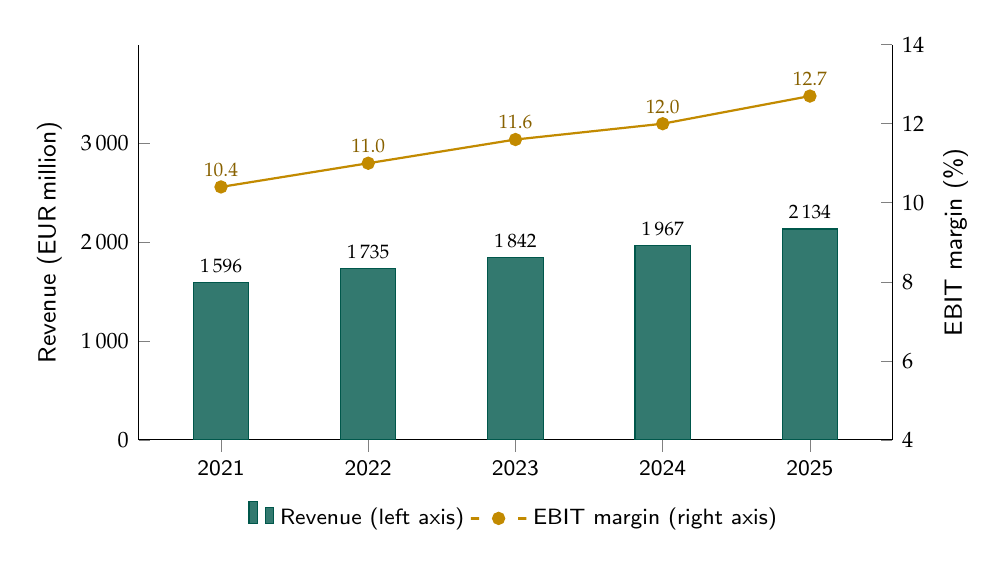
\begin{tikzpicture}
\begin{axis}[
    ybar, bar width=20pt, width=0.92\linewidth, height=6.6cm,
    ymin=0, ymax=4000, ytick={0,1000,2000,3000},
    symbolic x coords={2021,2022,2023,2024,2025}, xtick=data, enlarge x limits=0.14,
    ylabel={Revenue (\eur million)}, axis y line*=left, axis x line*=bottom,
    y tick label style={/pgf/number format/.cd, 1000 sep={\,}},
    tick label style={font=\sffamily\footnotesize}, label style={font=\sffamily\small},
    nodes near coords, nodes near coords style={font=\sffamily\scriptsize, /pgf/number format/.cd, 1000 sep={\,}},
    legend style={at={(0.5,-0.14)}, anchor=north, legend columns=2, font=\sffamily\footnotesize, draw=none, fill=none}]
  \addplot[fill=hgreen!80, draw=hgreen] coordinates {(2021,1596) (2022,1735) (2023,1842) (2024,1967) (2025,2134)};
  \addlegendentry{Revenue (left axis)}
  \addlegendimage{line legend, hgold, thick, mark=*}
  \addlegendentry{EBIT margin (right axis)}
\end{axis}
\begin{axis}[
    width=0.92\linewidth, height=6.6cm,
    ymin=4, ymax=14, ytick={4,6,8,10,12,14},
    symbolic x coords={2021,2022,2023,2024,2025}, enlarge x limits=0.14,
    axis y line*=right, axis x line=none, ylabel={EBIT margin (\%)},
    tick label style={font=\sffamily\footnotesize}, label style={font=\sffamily\small},
    nodes near coords, nodes near coords style={font=\sffamily\scriptsize, above, text=hgold!70!black,
      /pgf/number format/.cd, fixed, fixed zerofill, precision=1}]
  \addplot[hgold, thick, mark=*] coordinates {(2021,10.4) (2022,11.0) (2023,11.6) (2024,12.0) (2025,12.7)};
\end{axis}
\end{tikzpicture}
\captionof{figure}{Revenue (bars) and EBIT margin (line), 2021 to 2025. Revenue grew by 7.5\,\% a year on average.}
\end{center}

% ---- Segments ----------------------------------------------------------------------------------
\Needspace{16\baselineskip}
\section{Segment performance}
The group reports three segments. All three grew in 2025; Automation Systems contributed most of the increase
in revenue and earnings.

\sffamily\small
\begin{tabularx}{\linewidth}{@{}>{\raggedright\arraybackslash}X r r r r r@{}}
  \toprule
  \textbf{\eur million} & \textbf{Revenue 2024} & \textbf{Revenue 2025} & \textbf{Growth} & \textbf{EBIT 2025} & \textbf{EBIT margin} \\
  \midrule
  Automation Systems & 801 & 892 & +11.4\,\% & 128 & 14.3\,\% \\
  Industrial Components & 710 & 746 & +5.1\,\% & 94 & 12.6\,\% \\
  Service \& Aftermarket & 456 & 496 & +8.8\,\% & 71 & 14.3\,\% \\
  Corporate and consolidation & --- & --- & --- & $-$22 & --- \\
  \midrule
  \textbf{Group} & \textbf{1,967} & \textbf{2,134} & \textbf{+8.5\,\%} & \textbf{271} & \textbf{12.7\,\%} \\
  \bottomrule
\end{tabularx}
\rmfamily\normalsize

\textbf{Automation Systems} (41.8\,\% of group revenue) delivers controllers, drives and complete production lines
to machine builders and the automotive industry. \textbf{Industrial Components} (35.0\,\%) supplies bearings,
gears and couplings; growth was held back by weaker demand from the construction machinery market.
\textbf{Service \& Aftermarket} (23.2\,\%) provides maintenance contracts, spare parts and software updates. It is our most
resilient business and earns the same margin as Automation Systems.

% ---- Risks --------------------------------------------------------------------------------------------
\Needspace{22\baselineskip}
\section{Principal risks}
The Board reviews the principal risks twice a year. The table shows the five risks that could have the
greatest effect on our results, together with the main measures we take.

\sffamily\small
\begin{tabularx}{\linewidth}{@{}c >{\raggedright\arraybackslash}p{3.2cm} >{\raggedright\arraybackslash}X >{\raggedright\arraybackslash}p{1.6cm}@{}}
  \toprule
  \textbf{No.} & \textbf{Risk} & \textbf{How we respond} & \textbf{Trend} \\
  \midrule
  1 & Supply chain and input costs & Dual sourcing for critical electronic components; price clauses in 64\,\% of our contracts. & Stable \\
  2 & Customer concentration & Our ten largest customers account for 31\,\% of revenue; no single customer exceeds 7\,\%. & Falling \\
  3 & Cybersecurity & Annual external penetration tests; mandatory training for all 7,880 employees. & Rising \\
  4 & Regulation (energy efficiency, product liability) & Dedicated compliance team; product portfolio already meets the 2027 efficiency rules. & Rising \\
  5 & Currency exchange rates & 38\,\% of revenue is earned outside the euro area; we hedge about 70\,\% of expected net exposure twelve months ahead. & Stable \\
  \bottomrule
\end{tabularx}
\rmfamily\normalsize

% ---- Outlook -----------------------------------------------------------------------------------------------
\section{Outlook for 2026}
We expect global industrial production to grow moderately in 2026. Against this background we are guiding for:
\begin{itemize}[leftmargin=1.4em, itemsep=0.1em]
  \item \textbf{Revenue growth of 5 to 7\,\%}, including about 3 percentage points from the Brenner Sensorik acquisition;
  \item an \textbf{EBIT margin between 12.5 and 13.5\,\%};
  \item \textbf{capital expenditure of \eur 140 million}, compared with \eur 128 million in 2025;
  \item a payout ratio of \textbf{35 to 40\,\%} of net income, in line with our dividend policy.
\end{itemize}
These expectations assume stable exchange rates and no further escalation of trade restrictions. Should demand
weaken markedly in the second half, we have measures ready to protect profitability, but we would not
reduce our investment in research and development, which stood at 5.2\,\% of revenue in 2025.

\end{document}
